\documentclass[10pt,twocolumn,letterpaper]{article}

\usepackage{cvpr}
\usepackage{times}
\usepackage{epsfig}
\usepackage{graphicx}
\usepackage{amsmath}
\usepackage{amssymb}
\usepackage[euler]{textgreek}
\usepackage{multirow}
\usepackage{graphicx}
\usepackage{booktabs}

% Include other packages here, before hyperref.

% If you comment hyperref and then uncomment it, you should delete
% egpaper.aux before re-running latex.  (Or just hit 'q' on the first latex
% run, let it finish, and you should be clear).
\usepackage[pagebackref=true,breaklinks=true,letterpaper=true,colorlinks,bookmarks=false]{hyperref}

\cvprfinalcopy % *** Uncomment this line for the final submission

\def\cvprPaperID{****} % *** Enter the CVPR Paper ID here
\def\httilde{\mbox{\tt\raisebox{-.5ex}{\symbol{126}}}}

% Pages are numbered in submission mode, and unnumbered in camera-ready
\ifcvprfinal\pagestyle{empty}\fi
\begin{document}

%%%%%%%%% TITLE
\title{Severstal defect segmentation \\ IACV 2019-2020 Project} 

\author{Andrea Bionda\\
Politecnico di Milano\\
{\tt\small andrea.bionda@mail.polimi.it}}

\maketitle
%\thispagestyle{empty}

%%%%%%%%% ABSTRACT
\begin{abstract}
   Steel is one of the most important building materials of modern times. It was observed that the future of metallurgy requires the development of even more technological tools to face contemporary economic, ecological, and social challenges. 
   In order to increase efficiency in production, Severstal collected gigabytes of data looking for a deep learning approach that helps them in recognizing and classifying automatically surface defects on steel sheets.
   The goal of this challenge is not only to provide a good segmentation and classification of defects, but also an accurate classification between defective and non-defective images, in order to reduce false positives, and so waste of money and resources.
   In this paper, I will try to give a solution to the above problem, using a combination of two famous deep learning tools, named classification and segmentation respectively.
   The evaluation metrics used in this competition is the so called Dice coefficient, which is not only an accuracy index, but it also penalizes the false positives that the method finds, more similar to precision. (170)

   \textcolor{blue}{
   The abstract should be self contained and explain what the paper is about. Usually abstracts are no longer than 300 words. You should state what are the main contributions of your work and tempt the reader to continue to read your paper. A good abstract briefly describes your problem, approach, and key results. This document is based on the CVPR submission template, and it has been adapted to submit a technical report of a project of the Deep Learning and Image Classification course.}
\end{abstract}

%%%%%%%%% INTRODUCTION
%------------------------------------------------------------------------
\section{Introduction}
   The main contribution of this paper is to present a method to solve the above problem, that provides a good tradeoff between accuracy on defect segmentation and precision in defective-image identification. \\
   The proposed solution takes in input images of steel sheet that come from high-frequency cameras and output the same-size segmented images, which contain the area of the defect(s) identified (if any) and the corresponding type. \\
   The first explored approach is to use a single Fully Convolutional Neural Network that performs semantic segmentation over the four defects; in particular I have used the U-Net architecture. This method gives a Dice coefficient of 0.48 in the test set.
   In order to improve the precision, and so reducing false positives, the second and final approach is a pipeline of two different techniques: in the first stage, there is a Binary Classifier that is trained to filter out defect-free images; in the second stage, it is placed the segmentation model presented in the first method, that will segment only images that are labelled defective by the Classifier. This second approach gives a Dice coefficient of 0.71 in the test set. 


   \textcolor{blue}{
   This is the first section of your paper and you should contextualize the problem you are working on, why it is important, and give an overview of your results. It is useful to list all the contributions of your work very clearly, so that the reviewer can easily understand the value of your paper. This is helpful to guide the reader through the paper. If your project consists in replicating and/or extending another paper, then you should be very clear about it explaining what you did and how you proceeded.
   For instance, the main contribution of this paper are: 
   \begin{itemize}
      \item A brief tutorial on how to write a paper/technical report.
      \item Specific good/bad examples of writing.
      \item An example of structure that is suggested to follow for a technical report and can be reorganized as you need.
   \end{itemize}
   Each researcher has its own style and preferences when it comes to write a paper, so feel free to modify the structure as it pleases you. 
   This tutorial is especially directed to master students who might need more help to organize their reports.}

   \textcolor{blue}{
   \subsection{Language}
      All manuscripts must be in English. Do not use contraction forms, \eg \emph{doesn't} $\xrightarrow{}$ \emph{does not}, \emph{isn't} $\xrightarrow{}$ \emph{is not}. }

   \textcolor{blue}{
   \subsection{Paper length}
      Papers, excluding the references section, must be between \textbf{4-6} pages, bust must be no longer than \textbf{six pages}. The maximum number of pages is strict. Overlength papers will simply not be graded or graded negatively. Note that this \LaTeX\ guide already sets figure captions and references in a smaller font.
      The references section will not be included in the page count, and there is no limit on the length of the references section. For example, a paper of six pages with two pages of references would have a total length of 8 pages, so it is fine.}



%%%%%%%%% RELATED WORK
%------------------------------------------------------------------------
\section{Related work}
   Since the output of the problem is a pixel-wise label for the input image, it is essentially a semantic segmentation task. In our case, it is also used a binary classifier to refine the results.
   \subsection{U-Net}
      The baseline architecture used in the segmentation phase is the so called U-Net, that is composed of two concatenated parts: the contracting path (or down-sampling network or encoder network) works as a classical Fully Convolutional Neural Network (FCNN) to extract meaningful feature from the image, while the expansive path (or up-sampling network or decoder network) builds a high resolution output starting from the feature extracted during the first phase. The biggest contribution taken by this architecture is that each up-sampling layer is enriched with features information extracted in the corresponding downsampling layer network, in order to achieve higher semantic levels \cite{Unet}. 
   \subsection{Residual Networks} 
      This family of Convolutional Neural Network is built to face the degradation problem of very deep networks. The related paper proposes that such degradation is not caused by overfitting, but instead it is due to the well-known vanishing gradient issue. The main idea is to add an identity shortcut connection between blocks (group of convolutional layers), in such a way that each one learns features from both previous block and input value \cite{resnet}.
      In this paper, I will refer to ResNet34 and ResNet50, two models of the same family, but with different number of layers.
   \subsection{EfficientNet}
      The idea behind this family of Convolutional Neural Network is to scale a baseline model, called EfficientNet-B0, in width, depth, and resolution by a costant ratio, in order to obtain higher accuracy. This process allows to keep the number of parameters lower than the one in same accuracy-level models \cite{efficientnet}. In the proposed solution, I will refer to EfficientNet-B3, a good tradeoff between accuracy level and network size.

\textcolor{blue}{
In this section you should discuss published work that relates to your project. This is expected to be full of references, meaning that you have read the existing literature and you know what you are working on very well. This is not just a list or works, but you are not supposed to cluster papers that use similar approaches and compare them each other using very short sentences. I strongly suggest to check \cite{steinhardt, lipton} blog posts for some good practices in writing a paper. A quote that I like very much is \emph{``Research is spending 6 hours reading 35 papers, so you can write one sentence containing 2 references''} \cite{twit:ref}. Keep it in mind while you are writing!
}



%%%%%%%%% RELATED WORK
%------------------------------------------------------------------------
\graphicspath{ {./Resources/} }
\section{Dataset analysis}
   The first, and one of the most important phases of every Machine Learning task, is the analysis of input data. In this problem, we have 12568 greyscale images of size 1600x256x3, that come from real camera shot of steel sheets and a data file (.csv), that contains all the information in order to generate each defective mask. This dataset is obtained from the corresponding Kaggle competition \cite{Severstal}.The types of defects can be classified in Pitting (Figure \ref{fig:defect1}), Inclusion (Figure \ref{fig:defect2}), Scratches (Figure \ref{fig:defect3}) and Corrosion (Figure \ref{fig:defect4}).

   \begin{figure}[h]
      \centering
      \caption{Pitting} \label{fig:defect1}
      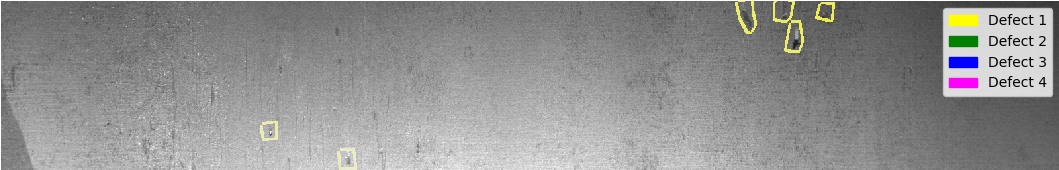
\includegraphics[scale=0.3]{Img_Defect1}
      \caption{Inclusion} \label{fig:defect2}
      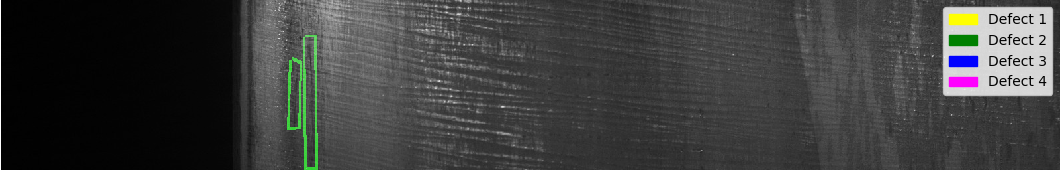
\includegraphics[scale=0.3]{Img_Defect2}
      \caption{Scratches} \label{fig:defect3}
      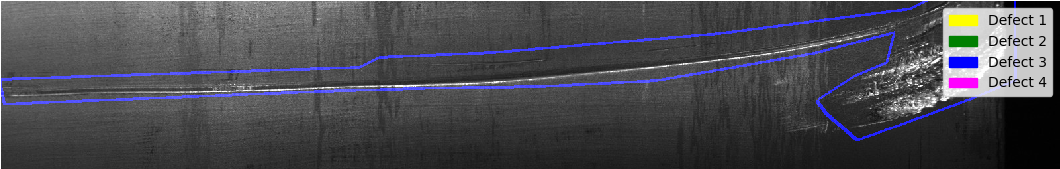
\includegraphics[scale=0.3]{Img_Defect3}
      \caption{Corrosion} \label{fig:defect4}
      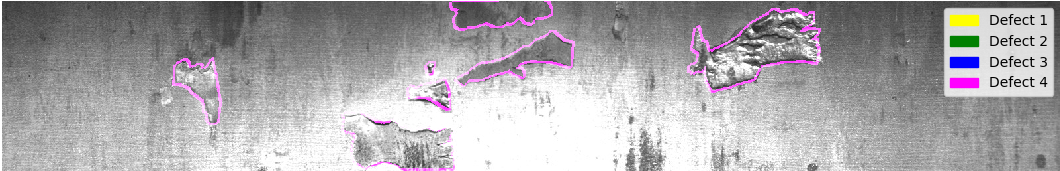
\includegraphics[scale=0.3]{Img_Defect4}
   \end{figure}

   The dataset exhibits a fairly even distribution between defective (56\%) and non-defective images (44\%), but among the defective ones we can notice a strong imbalance between defect classes (Figure \ref{fig:classImbalance}). This distribution can lead to recognize only one type of defect (the third one), since it represents the largest part of the defective images. During the discussion of the proposed approach, I will explain a solution to this problem.

   \begin{figure}[h]
      \centering
      \caption{Defect class distribution} \label{fig:classImbalance}
      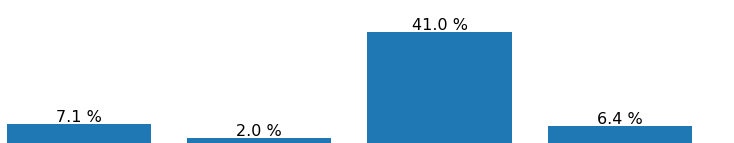
\includegraphics[scale=0.45]{Img_ClassImbalance}
   \end{figure}





%------------------------------------------------------------------------
\section{Proposed approach}
   The first and straightforward solution that I have applied to the problem is to build a U-Net architecture for semantic segmentation in such a way that it outputs same-size images with 4 channels, one for each defect class (Figure \ref{fig:firstApproach}).  
   Each channel (layer) of the output represents the heatmap (image where, for each pixel, a probability that it belongs to a defect in the original image is assigned) of the corresponding defect class. 

   \begin{figure}[h]
      \centering
      \caption{First approach: segmentation inference only} \label{fig:firstApproach}
      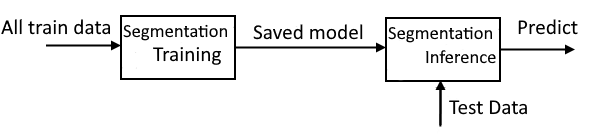
\includegraphics[scale=0.55]{Img_FirstApproach}
   \end{figure}

   This method has a very good capibility in defect recognition, but at the same time it hardly distinguishes real defects from the false ones, due to their similar pattern (an example on Figure \ref{fig:result1} and \ref{fig:result2}). This problem is highly penalized in the case in which no defects are present with Dice metric \eqref{eq:dice_loss}, that could be reasonable in high capacity foundries, where the goal is also to reduce at minimum the false scrap and so the waste of resources (if the machine labels part of the steel sheet as defective, it will be thrown away).\\
   For this reason, the second and real proposed approach is to train a Binary classifier for the purpose of distinguishing defective from non-defective images. The idea is to use the classifier to decide, during inference time, whether an image could contain a defect or not and, if the answer is true, to pass it to the U-Net to segment the defect, otherwise the segmentation inference is skipped and whole-zero masks are generated as heatmaps (Figure \ref{fig:secondApproach}).\\
   This pipeline will reduce the false scrap and increase Dice coefficient, as it is presented in the result section (Table \ref{table:res_finals}.).
    
   \begin{figure}[h]
      \caption{Proposed approach: pipelined inference } \label{fig:secondApproach}
      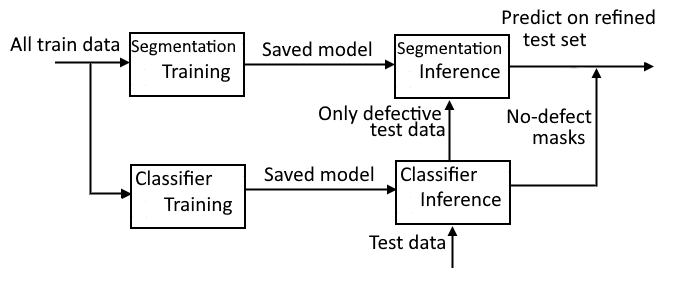
\includegraphics[scale=0.48]{Img_SecondApproach}
   \end{figure}


   \subsection{Multiclass Semantic Segmentation}
   The semantic segmentation task is performed by a U-Net based model. In my experiments, I have tried three different U-Net encoders: ResNet34, ResNet50 and EfficientNet-B3. In the following, I will refer to the EfficientNet-B3 model only since it has given the best result (Table \ref{table:res_encoders}.).
   The main advantage of using custom encoders is that it is possible to apply transfer-learning from pretrained weghts, allowing to transfer previous knowledge to the network. \\
   The encoder part follows the EfficientNet-B3 architecture \cite{efficientnet}. The decoder part, instead, is a classical U-Net expansion path, where each upsampling layer is concatenated with the corresponding downsampling one in the contracting part, followed by a block of Convolution, Batch-Normalization and ReLu layer. \\
   The decision about the right activation layer at the end of the network was a great challenge for quite a long time: even if Softmax is the straightforward choice for multiclass segmentation by definition, this means that I have to treat 'no Defect' pixels as a separate class altogether. In my opinion, this decision will stress even more the imbalanced data issue since for each pixel it is necessary to decide the right class, where, as I presented in the dataset analysis, it is clear that almost the entire amount of pixels belongs to the non-defective group. The usage of Sigmoid activation function, instead, brings the network to perform four \textit{one vs all} independent decisions, whether that pixel belongs to the corresponding class or not. The experiment results are inline with the above intuition (Table \ref{table:res_encoders})

   \subsection{Binary Classification}
   The classification task is delegated to a standard binary classifier. In my experiments I have tried two different models: ResNet34 and ResNet50. In the following, I will refer to ResNet50 only, because it has given the best result.
   The structure of the classifier follows the classical ResNet50 architecture \cite{resnet}, the last part of Fully Connected layers is removed and replaced by a Global Averaging Pooling layer attached with a sigmoid activation over the single binary output.



\textcolor{blue}{
This is the core of your paper, where you describe the details of the proposed method for solving the problem that you set up in the introduction. This is the most important section. It has to be clear why the chosen approach is the right thing to do with respect to the possible alternatives. The explanation of the method has to be readable and understandable and it should not raise obvious questions from the reader. 
You can divide the section in paragraphs or subsections that can be useful for the presentation of your method. Usually at this point you may want to place equations, figures and tables to clarify what you are explaining.
\subsection{Mathematics}
Please number all of your sections and displayed equations.  It is
important for readers to be able to refer to any particular equation.  Just
because you didn't refer to it in the text does not mean some future reader
might not need to refer to it.  It is cumbersome to have to use
circumlocutions like ``the equation second from the top of page 3 column
1''. 
\subsection{Footnotes}
Please use footnotes\footnote {This is what a footnote looks like.  It
often distracts the reader from the main flow of the argument.} sparingly.
Indeed, try to avoid footnotes altogether and include necessary peripheral
observations in
the text (within parentheses, if you prefer, as in this sentence).  If you
wish to use a footnote, place it at the bottom of the column on the page on
which it is referenced. Use Times 8-point type, single-spaced.
\subsection{References}
List and number all bibliographical references in 9-point Times,
single-spaced, at the end of your paper. When referenced in the text,
enclose the citation number in square brackets, for
example~\cite{Authors14}.  Where appropriate, include the name(s) of
editors of referenced books.
\subsection{Illustrations, graphs, and photographs}
All graphics should be centered.  Please ensure that any point you wish to
make is resolvable in a printed copy of the paper.  Resize fonts in figures
to match the font in the body text, and choose line widths which render
effectively in print.  Many readers (and reviewers), even of an electronic
copy, will choose to print your paper in order to read it.  You cannot
insist that they do otherwise, and therefore must not assume that they can
zoom in to see tiny details on a graphic.}




%------------------------------------------------------------------------
\section{Experiments}
   The entire pipeline is trained separately, so for legibility purpose I will divide the two experiments and then provide the final results using the Dice coefficient \eqref{eq:dice_loss}.
   \begin{equation}\label{eq:dice_loss}
      L_{dice} = \frac{2 * y_{pred} * y_{true}}{y_{pred} + y_{true}}
   \end{equation}
   \subsection{Segmentation}
      \paragraph{Data preparation}
         The first operation applied is to crop the images due to the large dimension of the input data and the corresponding limited amount of memory. Thanks to the idea behind Fully Convolutional Neural Network, it is possible to train and predict on different image dimension with good output resolution \cite{FCNN}.
         In order to apply a first level of data augmentation, the crop size varies on different epochs, also completely dark crops are prevented since does not bring any useful information. ??
         In order to face imbalanced dataset issue, the batch is composed of all images' classes in equal proportion (included non-defective class).

      \paragraph{Training parameters}
         \begin{itemize}
            \item Data augmentation is applied with both random spatial transformations (flip, rotation and shifting) and color augmentation (brightness and contrast).
            \item The crop size used are (5, 256, 384) and (5, 256, 512) that will interchange on epochs, where the first number in the tuple identifies the batch size.
            \item The loss function varies during the training: the first 70 epochs were trained using a balanced combination of two loss functions, Binary Cross Entropy and Dice \eqref{eq:dice_loss} that provides a tradeoff between accuracy and precision \eqref{eq:loss_bce_dice}. Finally the model is fine tuned for other 40 epochs using Tversky loss \eqref{eq:loss_tversky} with \textalpha=0.3 to reduce the false positive rate. 
            \begin{equation}\label{eq:loss_bce_dice}
               L_{bce\_dice} = L_{dice} + L_{bce}
            \end{equation}
            \begin{equation}\label{eq:loss_tversky}
               L_{Tversky} = \frac{TP}{TP + \alpha*FN + (1-\alpha)*FP}
            \end{equation}
            \item The network is optimized using Adam, with an initial learning rate of $ 10^{-3} $ that is reduced with a constant factor of 0.5 every time it reaches a plateau long three epochs.
         \end{itemize}

      \paragraph{Experimental results and observations}
         The followig results refer to tests on the segmentation model only.
         \begin{table}[h]
            \centering
            \begin{tabular}{||c c c||} 
            \hline
            Encoder model & Activation function & Dice metric\\ [0.4ex] 
            \hline\hline
            ResNet34 & Sigmoid & XXX \\ 
            \hline
            ResNet50 & Sigmoid & XXX \\
            \hline
            \textbf{EfficientNet-B3} & \textbf{Sigmoid} & \textbf{0.607} \\
            \hline
            EfficientNet-B3 & Softmax & XXX \\
            \hline
            \end{tabular}
            \caption{Results on different encoders and activation functions}
            \label{table:res_encoders}
         \end{table}

         As I mentioned before, U-Net provides a very accurate identification of defects, but hardly distinguishes real defects from false defects that usually are identified as small scarfs in the steel (Figure \ref{fig:result1}). 
         \begin{figure}[h]
            \centering
            \caption{Real (purple) vs False (blue) defects} \label{fig:result1}
            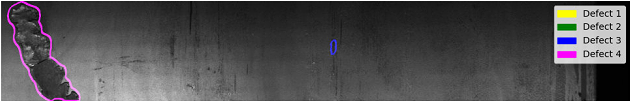
\includegraphics[scale=0.5]{Img_Result1.png}
         \end{figure}
         \\This would not be a big issue if the challenges' metrics do not penalize so much false defects on non-defective images, even if they are a small proportion of the entire image(Figure \ref{fig:result2}).  
         \begin{figure}[h]
            \centering
            \caption{False defects on good image} \label{fig:result2}
            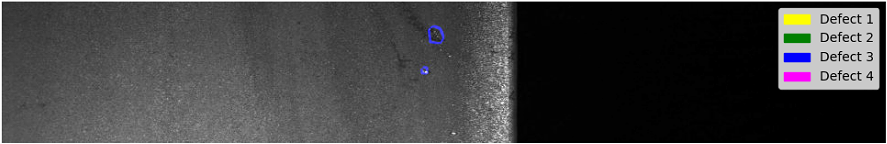
\includegraphics[scale=0.355]{Img_Result2.png}
         \end{figure}
   
   \subsection{Classification}
      \paragraph{Data preparation} 
         For classification I did not apply any data preprocessing.
                 
      \paragraph{Training parameters}
      \begin{itemize}
         \item Data augmentation is applied with both random spatial transformations (flip, rotation and shifting) and color augmentation (brightness and contrast).
         \item The images are fed on their original size of (4, 256, 1600), where the first number in the tuple identifies the batch size.
         \item The loss function is Binary Cross Entropy. 
         \item The network is optimized using Adam, with an initial learning rate of $ 10^{-3} $ that is reduced with a constant factor of 0.5 every time it reaches a plateau long three epochs.
      \end{itemize}

      \paragraph{Experimental results and observations}
         The followig results refer to tests on the classification model only.
         \begin{table}[!htb]
            \begin{minipage}{.5\linewidth}
               \begin{tabular}{cc|cc}
               \multicolumn{1}{c}{} &\multicolumn{1}{c}{} &\multicolumn{2}{c}{Predicted} \\ 
               \multicolumn{1}{c}{} & 
               \multicolumn{1}{c|}{} & 
               \multicolumn{1}{c}{True} & 
               \multicolumn{1}{c}{False} \\ \hline
               \multirow[c]{2}{*}{\rotatebox[origin=tr]{90}{Real}}
               & True  & 662 & 54   \\[1.5ex]
               & False  & 373   & 711 \\ \hline
               \end{tabular}
               \caption{Resnet34}
               \label{table:resnet34_cm}
            \end{minipage}%
            \begin{minipage}{.5\linewidth}
               \begin{tabular}{@{}cc|cc@{}}
               \multicolumn{1}{c}{} &\multicolumn{1}{c}{} &\multicolumn{2}{c}{Predicted} \\ 
               \multicolumn{1}{c}{} & 
               \multicolumn{1}{c|}{} & 
               \multicolumn{1}{c}{True} & 
               \multicolumn{1}{c}{False} \\ 
               \cline{2-4}
               \multirow[c]{2}{*}{\rotatebox[origin=tr]{90}{Real}}
               & True  & \textbf{695} & \textbf{21}   \\[1.5ex]
               & False  & \textbf{365}   & \textbf{719} \\ 
               \cline{2-4}
               \end{tabular}
               \caption{Resnet50}
               \label{table:resnet50_cm}
            \end{minipage} 
         \end{table} 
         As it can be seen from the confusion matrix above, the classification helps to identify most of the non-defective images and avoid the segmentation step, that in some cases can create only problems. The most important thing here is to keep the False Negative rate as small as possible, in order not to skip the segmentation of defective images.
            
   \subsection{Compelte pipeline}
      The training procedure of the entire pipeline is simply composed of the two procedures stated above.
      The following refers to the results coming from the two approaches, using EfficientNet-B3 as encoder model in the segmentation phase, and ResNet50 as binary classifier. 
      \begin{table}[h]
         \centering
         \begin{tabular}{||c c||} 
         \hline
         Approach & Dice coefficient\\ [0.5ex] 
         \hline\hline
         Segmentation only & 0.607 \\ 
         \hline
         \textbf{Complete pipeline} & \textbf{0.729} \\
         \hline
         \end{tabular}
         \caption{Results on different approaches}
         \label{table:res_finals}
      \end{table}


\textcolor{blue}{
In this section you validate your method showing the experiments that you performed. The experiments will vary depending on the project, but you might compare with previously published methods, perform an ablation study to determine the impact of various components of your system, experiment with different hyperparameters or architectural choices, use visualization techniques to gain insight into how your model works, discuss common failure modes of your model, etc. You should include graphs, tables, or other figures to illustrate your experimental results. Divide in subsections or paragraphs to help the reader navigate in your paper.
\paragraph{Datasets.}
Describe the data you are working with for your project. Usually you need to explain what type of data is it, how much data are you working with and if you applied any pre-processing, filtering, or other special treatment to use it. Remember that you have to cite each dataset you used in your project if it has been published from someone else. Instead, if you collected it by yourself you have to describe accurately how you gathered (and labeled) your data. 
\paragraph{Experiments setup.}
Here you describe all the architectural choices of your model, the hyper-parameters of your model, \eg optimizer, learning rate, momentum, batch size and if you cross-validate on them. 
\paragraph{Results and discussion.}
Discuss your results and compare with other methods. You can also perform an \emph{ablation study} on your model switching on and off some components to understand their contributions.
}



%-----------------------------------------------------------------------
\section{Conclusion} 
This project leverages the semantic segmentation and classification echniques to solve the steel defect detection problem. From the experiments arised that the combination of these two techniques works particularly weel as a tradeoff between accuracy and precision, in this particualar field.\\
Possible future improvements could be:
\begin{itemize}
   \item Try ensamble learning in order to exploit different encoder models in the final result.
   \item Fitht imabalanced dataset issue using a custom loss that takes in consideration the defect class distribution.
\end{itemize}

\textcolor{blue}{
Summarize your key results. What have you learned from the project and suggest future extensions or new applications of your ideas.}





%-------------------------------------------------------------------------
\section*{Acknowledgements}
Here you can thank all the people that have been helpful during the project, but are not coauthors. It is important to add this section only in the final version that you send to the professors and \textbf{NOT in the review version} in order to not compromise the double blind review process. We thank Andrea Romanoni for the insightful comments during the review of the manuscript, and all the old and new Gods who stand beside us when the deadline is dark and full of terrors. 

%-------------------------------------------------------------------------
\appendix
\section{Supplementary Material} 
Supplementary material is not counted toward your 4-6 page limit and should be submitted as a separate zip file. Your supplementary material might include:
\begin{itemize}
    \item Source code (if your project proposed an algorithm, or code that is relevant and important for your project.).
    \item Cool videos, interactive visualizations, demos, etc.
\end{itemize}

\paragraph{Examples of things to NOT put in your supplementary material}
\begin{itemize}
    \item The entire PyTorch/TensorFlow Github source code.
    \item Any code that is larger than 10 MB.
    \item Model checkpoints.
    \item A computer virus.
\end{itemize}




%-------------------------------------------------------------------------



{\small
\bibliographystyle{ieee}
\bibliography{egbib}
}

\end{document}
